\chapter{Functions and Relations}
\section{Relation}


\marginref{\raggedright\Cref{sec: ctp} \nameref{sec: ctp}}

\index{Relation}
\para{A relation between two sets \(A\), \(B\) is the subset of their \emph{cartesian
product} \(A \times B\).
Since, a cartesian product between \(A\) and \(B\) is also a set of the ordered pairs, so
is a relation \(R\),\[
    R \subseteq \{(a,b) \mid a \in A, b \in B\}
\]}

\para{There need not be any specific relation between the two elements. But often, it is useful
to talk about relations which employ a specific relationship between the two elements.
Hence, we can think of a relation as somehow connecting the two elements.}
\para{A relation on a set \(A\) is simply the subset of \(A \times A\).}

\begin{example}
    Consider sets \(A = \{2, 4, 6, 8, \dots\}\) and \(B = \{1,3,5,7,9,\dots\}\). Let \(R\) be
    the relation such that, \[R = \{(a,b) \mid a,b \text{ are divisible by 3 and}, a \in A, b \in B\}\]
    This relation is simply the set of all multiples of \(3\).
\end{example}
\begin{example}
    \label{ex: reltri}
    Let \(A = \{1,2,8\}\), \(B = \{3,5,6\}\). Let \(R\) be the relation, \[
        R = \{(a,b) \mid a > b, a \in A, b \in B\}
    \]
    Then \(R\) contains the ordered pairs \((8,3)\), \((8,5)\) and \((8,6)\)
\end{example}
\para{We show that \((a,b) \in R\) by saying \(a R b\).}

\begin{figure}[H]
    \centering
    \scalebox{.7}{\incfig{relation}}
    \caption{Pictorial representation of \Cref{ex: reltri}}
\end{figure}

\subsection{Domain}
\index{Relation!domain}
\para{The domain of a relation \(R \subseteq A \times B\) is the set of all first elements of 
the ordered pairs of the relation, that are in set \(A\). \[D_R = \{a \mid (a,b) \in R\}\]}

\subsection{Range and Co-domain}

\subsubsection{Range}
\index{Relation!range}
\para{Range of \(R\) is the set of all second elements of the ordered pairs in the relation, that
are in set \(B\). \[Range_R = \{b \mid (a,b) \in R\}\]}


\marginnote{You may note that \(Range_R \subset Co-domain_R\)}

\subsubsection{Co-domain}
\index{Relation!co-domain}
\para{Co-domain of \(R \subseteq A \times B\) is the set \(B\) itself.} 

\section{Types Of Relations}

\para{Although it might seem like discussing the type of relations would be as trivial as sets,
there are actually a couple really important type of relations. I'll mention the ones
we really need to know about.}

\subsection{Trivial Types}

\para{Mainly, these are trivial in the way that they're of very low importance to us. The ones
that are useful later, have been especially marked.}

\subsubsection{Empty Relation}

\para{The relation \(R\) is an empty relation if it does not contain any elements.
\(R = \varnothing \subset A \times B\).}

\subsubsection{Universal Relation}

\para{Yes, it is the relation that contains all the elements. A universal relation \(R\) on \(A\)
is \(R = A \times A\).}

\subsubsection{Inverse Relation}
\index{Relation!Inverse}

\para{Let \(R\) be the relation from \(A\) to \(B\). Then \(R\inv\) is the relation from \(B\)
to A such that, \[R\inv = \left\{ (b,a) \mid (a,b) \in R \right\}\]
Therefore, we may have \((a,b) \in R \iff (b,a) \in R\inv\).}

\subsubsection{Identity Relation}
\index{Relation!Identity}

\para{The identity relation \(I_A\) on \(A\) is defined as
\[
    I_A = \left\{(a,a) \mid a \in A\right\}
\]}

\subsection{Equivalence Relation}

\subsubsection{Reflexive relation}

\marginnote{All identity relations are reflexive relations but all reflexive relations are
not identity relations. See \Cref{ex: identity}.}

\para{A relation \(R\) is a reflexive relation on \(A\), if for every \(a \in A\),
\((a,a) \in R\).}

\index{Relation!Reflexive}

\begin{example}
    \label{ex: identity}
    The relation \(I_A = \left\{(1,1), (2,2), (3,3)\right\}\) is an identity relation on the set
    \(A = \left\{1,2,3\right\}\). \\
    However, the relation \(R = \left\{(1,1), (2,3)(3,2), (2,2), (3,3)\right\}\)
    is not an identity relation on \(A\), but rather a reflexive relation. But \(I_A \subset R\).\par
    Here, \(R\) is a reflexive relation but not an identity relation.
\end{example}

\subsubsection{Symmetric Relation}
\index{Relation!Symmetric}

\para{A relation \(R\) on \(A\) is symmetric if \((a,b) \in R \iff (b,a) \in R\).}

\begin{example}
    Let \(R\) be the relation on \(\RR\) such that \[
        R = \left\{(x,y) \mid x + y = 5\right\}
    \]
    This relation is symmetric, because suppose any two reals \(x\) and \(y \in R\). Then,
    \(x + y = 5\). But since addition is commutative, \(x + y = y + x = 5\). 
    Thus, \((x,y) \in R \iff (y,x) \in R\).
\end{example}

\subsubsection{Transitive Relation}
\index{Relation!Transitive}

\para{A relation \(R\) on \(A\) is transitive if \((a,b) \in R\) and \((b,c) \in R \implies (a,c) \in R\). }

\begin{example}
    The relation \(<\) is a transitive relation on \(\RR\). For instance, if \(a < b\), \(b < c\),
    then \(a < c\).
\end{example}

\subsubsection{Equivalence Relation}
\index{Relation!Equivalence}

\para{An equivalence relation on \(A\) is a relation that is transitive, reflexive, and symmetric.}

\marginnote{If you haven't already noticed, I have deliberately chosen examples that
are non-conventional. I have done it in order to showcase that relations can be anything!}

\begin{example}
    The relation `\(=\)' is an equivalence relation on \(\RR\). It is symmetric as \(a = b \iff b = a\). 
    It is reflexive as \(a = a\). It is transitive as \(a = b, b = c \implies a = c\).
\end{example}

\section{Functions}

\para{Functions are a special type of relation. They're, for most cases, much more useful
than relations for us.}

\index{Function}

\begin{definition}
    \label{def: function}
    A function from \(A\) to \(B\) is a set of ordered pairs, \[
        f = \left\{(a,b) \mid a \in A, b \in B, \text{ for every } a \in A, \text{ there
        exist one and only one } b \in B \right\}
    \]
\end{definition}

\index{Function!Pre-image}
\index{Function!Image}

\para{A little more informally, functions are a mapping from set \(A\) to \(B\). We represent
this by saying \(f \colon A \rightarrow B\). When we map \(a \in A\) to \(b \in B\),
we say that \(b\) is the `image' of \(a\) under \(f\) and \(b\) is called the `preimage' of 
\(a\) under \(f\). We may represent that \(f\) maps \(a\) to \(b\) as \(a \mapsto b\).
Alternatively, and more commonly, \(f(a) = b\).}

\begin{figure}[H]
    \begin{subfigure}{.5\textwidth}
        \centering
        \incfig{func}
        \caption{A function from \(A\) to \(B\).}
    \end{subfigure}%
    \begin{subfigure}{.5\textwidth}
        \centering
        \incfig{func2}
        \caption{Also a function, note that \(h\) doesn't have a pre-image.}
    \end{subfigure}
    \begin{subfigure}{.5\textwidth}
        \centering
        \incfig{notfunc}
        \caption{Not a function, \(d\) has no image.}
    \end{subfigure}
    \begin{subfigure}{.5\textwidth}
        \centering
        \incfig{notfunc2}
        \caption{Also not a function because \(d\) has two images.}
    \end{subfigure}
    \caption{Some examples of functions and not functions.}
\end{figure}

\subsection{Domain and Range}

\subsubsection{Domain}

\para{From the little use of `every' in \Cref{def: function}, you may realise that every element
of \(A\) has an image, i.e. every element in \(A\) is included in the ordered pairs of a function
\(f\). Thus, the domain of a function \(f : A \rightarrow B\) is the whole set \(A\).}

\subsubsection{Range and Co-domain}

\para{For a function \(f : A \rightarrow B\), the co-domain is the set \(B\). The Range
for \(f\) is the \emph{set of all images of pre-images.}}

\begin{example}
    For \(f \colon \RR \setminus \left\{0\right\} \to \RR\) such that \(f(x)=\dfrac{1}{x}\). The Range
    is \(\RR \setminus \left\{0\right\}\), as is the domain. The Co-domain is \(\RR\).
\end{example}

\subsection{Informal Definition}

\index{Variable!Dependent}
\index{Variable!Independent}
\para{A function can also be thought of a machine that takes in an independent variable and churns
out a dependent variable. This is a very vague abuse of already known ideas to somehow understand
the abstractness of the idea of a function.}

\begin{figure}[H]
    \centering
    \scalebox{0.6}{\incfig{depindep}}
    \caption{Dependent and Independent variables}
\end{figure}

\subsection{Implicit and Explicit}

\subsubsection{Explicit Function}
\index{Function!explicit}
\para{When we can clearly write out the dependent variable in terms of the independent variable,
the function is called Implicit.}

\begin{example}
    \(f(x) = y = x^3\) is an explicit function since it can be written with only the help of \(x\).
\end{example}

\subsubsection{Implicit Function}
\index{Function!implicit}
\para{These are the functions in which the dependent variable cannot be written only in the terms
of the independent variable.}

\begin{example}
    \(x^3y^2 + x - y + xy =0\) is an Implicit function. It may be represented as \(R(x,y) = 0\).
\end{example}

\subsection{Digression}
\irrev

\para{The functions we have considered till now are only real valued, and we have confined ourselves
to a single-variable being independent. Really, the title of this part is wrong and should be more
accurately Single-Variable Calculus.}
\para{The notions of implicit and explicit are quite annoying too,
which are better dealt with in Multi-Variable Calculus. We will not release ourselves of this confinement
for the rest of the part as it is irrelevant for JEE. But beware, you will know only a half of 
only Calculus even after JEE, let alone anything in Mathematics.}

\subsection{Bounded Functions}

\index{Function!bounded}
\index{Function!unbounded}

\para{A function is bounded if it is bounded from both above and below. A real-valued function, \(f : A \rightarrow B\) is bounded
from above if for each \(a \in A\), \(f(a) \le M\). It is bounded from below if for each \(a \in A\),
\(f(a) \ge N\).}
\para{Thus, a bounded function \(f\) lies in the interval \(\left[M,N\right]\). It may also lie on
any interval of the same kind, i.e \((M,N)\), \(\left[M,N\right)\), or \(\left(M,N\right]\).}

\begin{example}
    [Bounded Functions]
    Some examples of bounded functions are:
    \begin{enumerate}
        \ii \(\sin(x), \cos(x) \in \left[-1,1\right]\)
        \ii \(\dfrac{1}{x^2} \in \left(0,\infty\right)\)
    \end{enumerate}
\end{example}

\begin{example}
    [Unbounded functions]
    Some examples of unbounded functions are:
    \begin{enumerate}
        \ii \(\csc(x), \sec(x) \in \left(-\infty, -1\right] \cup \left[1, \infty\right)\)
        \ii \(\tan(x), \cot(x) \in \left(-\infty, \infty\right)\)            
    \end{enumerate}
\end{example}

\section{The ``...'' function}
\label{sec: pedantic}
\irrev
\para{From this point we make many mentions of the ``sine'' function, the ``cosine'' function,
and so on. However, there is no ``sine'' function. People generally call the function \(f\),
such that \(f(x) = \sin(x)\) as the sine function. What they really mean is the function that maps
\(x\) to \(\sin(x)\). However, because of lack of notation and convenience, we refer to it 
as the ``sine'' function which is just an abuse of notation. ``\(\sin(x)\)'' is not a function. It is
just a number. This is just some nitpicking.}

\section{Graphing the Function}
\index{Function!graph}
\para{Consider any function \(f\) that maps from \(x\) to \(y\), where any \(a\) is literally 
anything. It could be \(x^3\), \(\sin(x)\), or \(e^x\). Basically, \(y = f(x)\). If we map
\(x\) and \(y\) as co-ordinates on the cartesian plane, we get the graph of the function, \(f\)
such that \(f(x) = y\).}

\begin{figure}[H]
    \centering
        \begin{tikzpicture}
            \begin{axis}[funcgraph]
                \addplot[domain=-5:5,samples=100,red]{sin(deg(x))};
            \end{axis}
        \end{tikzpicture}
        \caption{Graph of the function ``{\color{red}\(\sin(x)\)}''}

\end{figure}

\subsection{Vertical Line Test}

\index{Function!Vertical Line Test}

\para{When we map \(f\) onto the cartesian plane, because of the very definition of a function,
there are no two ordered pairs \((x,a)\) and \((x,b)\) since \(x\) cannot have two images.
Because of this, if we draw a vertical line at any \(x\) for the function \(f\), it must pass 
only once (since there is only \(y\) for one \(x\)). We can use this test to determine 
through the graph of any relation, whether it is a function or not. This is called the vertical line
test.}

\begin{figure}[H]
    \begin{subfigure}{0.5\textwidth}
        \centering
        \begin{tikzpicture}[scale=1]
            \begin{axis}[funcgraph]
            \draw [blue] (axis cs:3,-10)--(axis cs:3,10);
            \addplot[domain=-3:3,red,samples=50]({x^2},{x});
            \end{axis}
        \end{tikzpicture}
    \caption{Not a function}
    \end{subfigure}%
    \begin{subfigure}{.5\textwidth}
        \centering
        \begin{tikzpicture}[scale=1]
            \begin{axis}[funcgraph]
                \addplot[red]{x^2};
            \draw [blue] (axis cs:3,-1000)--(axis cs:3,1000);
            \end{axis}
        \end{tikzpicture}
        \caption{A function}
    \end{subfigure}
    \caption{{\color{blue}Vertical Line test} for {\color{red}functions}}
\end{figure}

\para{Here are the graphs of some elementary algebraic functions. Their domain and range are listed
in the caption, where \(D\) is the domain, and \(R\) the range.}

\begin{figure}[H]
    \centering
    \label{fig: functs}
    \begin{subfigure}{.5\textwidth}
        \centering
        \begin{tikzpicture}
            \begin{axis}[funcgraph]
                \addplot[red,domain=-10:10]{3} node[above,blue,pos=0.7] {$y=c$};
            \end{axis}
        \end{tikzpicture}
    \caption{Constant function, \(D = \RR\), \(R = \left\{c\right\}\)}
    \end{subfigure}%
    \begin{subfigure}{.5\textwidth}
        \centering
        \begin{tikzpicture}
            \begin{axis}[funcgraph]
                \addplot[red,domain=-10:10]{x} node[left,blue,pos=0.7] {$y=x$};
            \end{axis}
        \end{tikzpicture}
    \caption{Identity Function, \(D = \RR\), \(R = \RR\)}
    \end{subfigure}

    \begin{subfigure}{.5\textwidth}
        \centering
        \begin{tikzpicture}
            \begin{axis}[funcgraph]
                \addplot[red,domain=-10:10]{x^2} node[left,blue,pos=0.7] {$y=x^2$};
            \end{axis}
        \end{tikzpicture}
    \caption{Square Function, \(D = \RR\), \(R = \RR^+ \cup \left\{0\right\}\)}
    \end{subfigure}%
    \begin{subfigure}{.5\textwidth}
        \centering
        \begin{tikzpicture}
            \begin{axis}[funcgraph]
                \addplot[red,domain=-2:2]{x^3} node[left,blue,pos=0.7] {$y=x^3$};
            \end{axis}
        \end{tikzpicture}
    \caption{Cubic Function, \(D = \RR\), \(R = \RR\)}
    \end{subfigure}

    \begin{subfigure}{.5\textwidth}
        \centering
        \begin{tikzpicture}
            \begin{axis}[funcgraph]
                \addplot[red,domain=0.01:1,samples=100]{1/x}  node[right,blue,pos=0.7] {$y=\dfrac{1}{x}$};
                \addplot[red,domain=-1:-0.01,samples=100]{1/x};
            \end{axis}
        \end{tikzpicture}
    \caption{Reciprocal Function, \(D = \RR \setminus \left\{0\right\}\), \(R = \RR \setminus \left\{0\right\}\) } 
    \end{subfigure}%
    \begin{subfigure}{.5\textwidth}
        \centering
        \begin{tikzpicture}
            \begin{axis}[funcgraph]
                \addplot[red,domain=-10:-0.01]{-x};
                \addplot[red,domain=0.01:10]{x} node[right,blue,pos=0.4] {$y=\abs{x}$};
            \end{axis}
        \end{tikzpicture}
    \caption{Modulus Function, \(D = \RR\), \(R = \RR^+ \cup \left\{0\right\}\)}
    \end{subfigure}
\caption{Some Elementary Functions}
\end{figure}

\section{Identical Functions}

\para{Two functions, \(f\), \(g\) are said to be identical if and only if,}

\begin{itemize}
    \ii Domain of both functions are equal, \(D_f = D_g\).
    \ii Range of both functions are equal, \(R_f = R_g\).
    \ii \(\forall x \in D_f\) or \(D_g\), \(f(x) = g(x)\).
\end{itemize}

\begin{example}
    \(f(x) = x\) and \(g(x) = \dfrac{1}{1/x}\) are identical for 
    \(x \in \RR \setminus \left\{0\right\}\).
\end{example}

\section{Piecewise functions}

\index{Function!Piecewise}

\para{When a function \(f\) of \(x\) has a different formula for particular intervals of \(x\),
we call it a piecewise function. We represent it as, \[
    \begin{cases}
        F & \phi(x) \\
        G & \varphi(x) \\
        \vdots & \vdots \\
        Z & \pi(x) \\
    \end{cases}
\]
Where each of the 

}
\begin{example}
    The modulus function, \(y = \abs{x}\) is a piecewise function:
    \[
    \begin{cases}
        x & x > 0\\
        0 & x = 0\\
        -x & x < 0\\
    \end{cases}
\]
\end{example}

\section{Algebra of Functions}

\para{Let \(f : A \rightarrow \RR\), \(g : A \rightarrow \RR\) be two functions where 
\(A \subset \RR\). Then, we have,
\begin{enumerate}
    \ii \(f + g : A \rightarrow \RR\), \((f + g)(x) = f(x) + g(x)\), for \(x \in A\).
    \ii \(f - g : A \rightarrow \RR\), \((f - g)(x) = f(x) - g(x)\), for \(x \in A\).
    \ii \(f \cdot g : A \rightarrow \RR\), \((f \cdot g)(x) = f(x) \cdot g(x)\), for \(x \in A\).
    \ii \(\dfrac{f}{g} : A \rightarrow \RR\), \(\dfrac{f}{g}(x) = \dfrac{f(x)}{g(x)}\), for \(x \in A\),
    given than \(g(x) \ne 0\) for all \(x \in A\).
\end{enumerate}}

\section{Exponential/Power Functions}

\index{Function!power}
\index{Function!exponential}

A function \(f\) such that \(x \xmapsto{f} e^x\) or more compactly \(f(x) = e^x\) is called
the exponential functional. A pedantic point much in spirit of \cref{sec: pedantic} 
is that \(f(x)\)
is not a function, it is a value. We'll henceforth sometimes omit this, but also refrain ourselves
from going as far as to call ``\(y = f(x)\)'' a function. 

For some reason, JEE seems fond of calling power function \(f\) such that \(f(x) = a^x\) an 
exponential function. I'll try to avoid collisions of the two different things, but just 
entertain this weird notion for a moment.
\parbreak

Whenever we write the function \(a^x\) we assume two implicit conditions, \begin{inparaenum}[1)]
    \ii that \(a > 0\), \(a\) is non-negative,
    \ii and that \(a \ne 1\).
\end{inparaenum}

The reason for adopting such convention is that \(a^x\) has a nice domain. If \(a\) were to
be negative, defining the domain would be quite annoying. It also helps in ensuring that 
\(a^x\) is not a constant function, the cases \(a = 0\) and \(a = 1\).

Thus, for the function \(a^x\), \(a \in \left(0,1\right) \union \left(1, \infty\right)\). This
divides the values of \(a\) into two intervals. In-fact for these intervals, \(a^x\) behaves 
differently!

\subsection[Case I]{\(\mathbf{0 < a < 1}\)}

The function \(a^x\) is in such case decreasing. A function is decreasing if \(f(x_1) \ge f(x_2)
\iff x_1 \le x_2\). It is possible to draw the graph of the function by considering
values of \(x\) for some specific \(a\). But I'll just show the graph. Also, it is decreasing 
because if \(0 < a < 1\), then it is easy to see that for larger values of \(x\), \(a^x\) decreases.

\begin{figure}[H]
    \centering
    \begin{tikzpicture}
        \begin{axis}[funcgraph]
            \addplot [red, domain=-2:2] {0.4^x} node [right,blue,pos=1/2] {$a^x$};
        \end{axis}
    \end{tikzpicture}
\end{figure}

 Clearly, for \(0 < a < 1\), \(a^{g(x)} \ge a^{f(x)} \iff g(x) \le f(x)\). The inequality flips. 
 in some manner. This is simply because of the earlier stated decreasing nature of the function.
 
 Inequalities of such kind are called exponential inequalities. The domain \(D_f = \RR\) and
 the range is \(R_f = \RR^+ = (0, \infty)\). 

 \subsection[Case II]{\(\mathbf{a > 1}\)}

 Contrastingly to our above function, this function is increasing, for \(x_1 \ge x_2\) it is easy
 to see that \(a^{x_1} \ge a^{x_2}\). 

 \begin{figure}
    [H]
    \centering
    \begin{tikzpicture}
        \begin{axis}
            [funcgraph]
            \addplot [red, domain=-2:2] {2.5^x} node [left, blue, pos=1/2] {$a^x$}; 
        \end{axis}
    \end{tikzpicture}
 \end{figure}

 Also, clearly here, \(a^{g(x)} \ge a^{f(x)} \iff g(x) \ge f(x)\). Simply because the function is 
increasing. The inequality remains the same when comparing exponents. The domain and range
are the same as above. 

\begin{remark}
    Note that the usual properties of exponents that we are familiar with, \((a^{b})^{c} = a^{bc}\)
    and of the same kind only work for \(b, c\) being positive integers. For example, consider
    \((-8)^{1/3} = (-8)^{2/6} = 64^{1/6} = 2\) but clearly \(-8^{1/3}\) is \(-2\). Beware.
\end{remark}

\section{The Logarithm function}

The function \(f\) of the form \(f(x) = \log_{a} x\) is a logarithmic function. Much like 
the exponential function, it is defined for \(a > 0\) and \(a \ne 1\). Unlike the exponential, 
however, it also has the condition \(x > 0\). In-fact, \(\log_{a} x = y \iff a^y = x\). Clearly,
from here we have \(x > 0\). We may again divide up it into two intervals.

Briefly, for \(0 < a < 1\), it is a decreasing function. You can check that for 
some discrete values. For \(a > 1\) it is an increasing function. The domain in
both cases is \(D_f = (0, \infty)\) and the range is \(R_f = \RR\). 

\begin{figure}
    [H]
    \centering 
    \begin{subfigure}{0.5\textwidth}
        \begin{tikzpicture}
            \begin{axis}
                [funcgraph]
                \addplot [red, domain = 0.02:2,samples=100] {log10(x)/log10(0.4)};
            \end{axis}
        \end{tikzpicture}
        \caption{\(0 < a < 1\)}
    \end{subfigure}%
    \begin{subfigure}{0.5\textwidth}
        \begin{tikzpicture}
            \begin{axis}
                [funcgraph]
                \addplot [red, domain = 0.02:2,samples=100] {log10(x)};
            \end{axis}
        \end{tikzpicture}
        \caption{\(a > 1\)}
    \end{subfigure}
\end{figure}

Anyways, the same thing happens with inequalities as it did with the exponential,
for \(\log_{a}f(x) \ge \log_{a} g(x)\), if \(0 < a < 1\), \(f(x) \le g(x)\). And if
\(a > 1\), \(f(x) \ge g(x)\). 

Also, 
\[
    \begin{cases}
        log_{a} x \ge 0 \iff x \ge 1 \mid a > 1 \\
        log_{a} x \ge 0 \iff 0< x \le 1 \mid 0 < a < 1 \\
    \end{cases}
\]

\begin{proposition}
    Some properties of logarithm for \(a \in \RR_{>0} \setminus \left\{1\right\}. \) and
    \(m, n \in \RR\).  
    \begin{enumerate}
        \ii \(\log_{c}(ab) = \log_{c}\abs{a} + \log_{c}\abs{b}\)
        \ii \(\log_{c}\dfrac{a}{b} = \log_{c}\abs{a} - \log_{c}\abs{b}\)
        \ii \(\log_{c}{a^b} = b\log_{c}{a}\)
        \ii \(\log_{c^b}{a} = \dfrac{1}{b}\log_{c}{a}\)
        \ii \(\log_{c}p = \dfrac{1}{\log{p}c}\)
        \ii \(a^{\log_{c}b} = b^{\log_{c}a}\)
    \end{enumerate}
\end{proposition}

\section{Some other functions}

\subsection{Greatest Integer Function}

The greatest integer function or the floor function, \(\floor{\bullet} : \RR \to \ZZ\) is defined
as,
\index{Function!Greatest Integer Function}
\begin{definition}
    [Floor]
    \[
        \floor{x} = a \mid a \le x < a + 1, a \in \ZZ
    \]
\end{definition}

The symbol for floor/GIF is for some reason, mostly \([\bullet]\) in JEE. In any case, they
generally mention the symbol in the question.

Therefore, for \(x \in [a,a+1)\), where \(a \in \ZZ\), \(\floor{x} = a\). Using this
definition, and setting up values of \(a\), we have the following graph,

\begin{figure}
    [H]
    \centering
    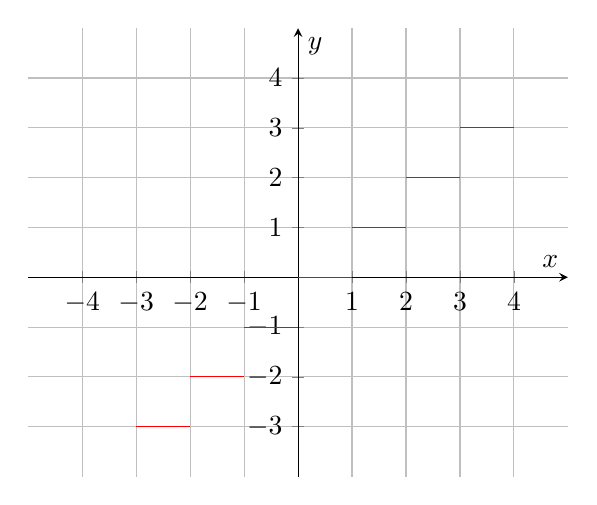
\begin{tikzpicture}
        \begin{axis}
            [ axis lines=middle,
            grid=major,
            xmin=-5,
            xmax=5,
            ymin=-4,
            ymax=5,
            xlabel=$x$,
            ylabel=$y$,
            xtick={-4,-3,...,4},
            ytick={-3,-2,-1,...,4},
            legend style={
            at={(rel axis cs:0,1)},
            anchor=north west,draw=none,inner sep=0pt,fill=gray!10}]
            \addplot[red, domain=-3:-2]{-3};
            \addplot[red, domain=-2:-1]{-2};
            \addplot[red, domain=-1:0]{-1};
            \addplot[red, domain=0:1]{0};
            \addplot[red, domain=1:2]{1};
            \addplot[red, domain=2:3]{2};
            \addplot[red, domain=3:4]{3};
        \end{axis}
    \end{tikzpicture}
\end{figure}

The end points of each \emph{step} are open. 

Some properties of floor are,

\begin{proposition}
    For \(x \in \RR\) and \(n, a, b \in \ZZ\),
    \begin{enumerate}
        \ii \(\floor{x} + \floor{-x} = 0 \mid x \in \ZZ\)
        \ii \(\floor{x} + \floor{-x} = -1 \mid x \notin \ZZ\)
        \ii \(a \le \floor{x} \le b \iff a \le x < b + 1\)
        \ii \(\floor{x} > n \iff x \ge n + 1\) 
    \end{enumerate}
\end{proposition}

\section{Injective, Surjective and all that}

\subsection{Injective}

\index{Function!Injective}

\para{If for all \(x \in A\), for function \(f : A \rightarrow B\), \(x\) has a `distinct' image,
the function is called one-one or injective. What it means is that any image has only one pre-image
under \(f\). Therefore, \(f(a) = f(b) \iff a = b\). Since, \(f(a)\) and \(f(b)\) must have only
one pre-image. Since they're the same, the pre-image must also be the same.}

\index{Function!Many-One}

\para{If this is not the case, any image may have more than one pre-image under \(f\),
the function is not injective and is called many-one. Here, \(f(a) = f(b) \notiff a = b\).}

\begin{figure}[H]
    \begin{subfigure}{.5\textwidth}
        \centering
        \begin{tikzpicture}
            \begin{axis}[funcgraph]
                \addplot[domain=-10:10,red]{x^2};
            \end{axis}
        \end{tikzpicture}
        \caption{ {\color{red}\(x^2\)}, a many-one function}
    \end{subfigure}%
    \begin{subfigure}{.5\textwidth}
        \centering
        \begin{tikzpicture}
            \begin{axis}[funcgraph]
                \addplot[domain=-10:10,blue]{x^3};
            \end{axis}
        \end{tikzpicture}
        \caption{{\color{blue}\(x^3\)}, a one-one function}
    \end{subfigure}
    \caption{{\color{blue}One-one} and {\color{red}Many-one} functions}
\end{figure}

To determine whether a function is one-one or many-one, we may either draw the 
graph of the function, and check if it is one-one by drawing a horizontal line,
if it cuts it at more than one place, then the function is clearly many-one.

The other method is to check whether \(f(x_1) = f(x_2) \iff x_1 = x_2 \) but is usually
difficult.
The last method uses differentiation and should be skipped for now,
for a continuous function, \(\forall x\), \(f^\prime(x)\) must have the same sign, i.e,
it must be either \(\ge 0\) or \(\le 0\). The solutions of \(f^{\prime} (x) = 0\) must
not form an interval. Do not use for functions not continuous over \(\RR\). 

\begin{remark}
    If a function \(f : A \to B\) is injective, then \(n(A) \le n(B)\). Thus,
    \(B\) is \emph{at least} as large as \(A\).
\end{remark}

\subsection{Surjective}

\index{Function!Surjective}
\index{Function!Into}

Let \(f\) be a function, \(f : A \to B\). If the range of \(f\) is equal to \(B\),
the co-domain, then \(f\) is surjective. The basic idea is that,

\[
    \forall y \in B, \exists x \in A \mid f(x) = y
\]

So, each \(y \in B\) has a pre-image. Functions that are surjective are also called
\emph{onto}. The functions that are not surjective are \emph{into}.

To determine if a function is surjective, we may use two methods. One is
to figure out the range, if it is the same as the co-domain then it is surjective. 
The other method is to show that \(f(g(y) = y)\). If now we show
that \(g(y)\) is defined for all \(y \in B\) and \(g(y) \in A\). Then, \(f\) is
surjective.

\begin{remark}
    If \(f : A \to B\) is surjective, then \(n(A) \ge n(B)\). The size of \(B\)
    is at most equal to \(A\).
\end{remark}

\subsection{Bijection}

If a function is both injective and surjective, then it is bijective.
Formally, \(\forall y \in B\) there is \emph{exactly} one \(x \in A\) such that
\(f(x) = y\). 

From the earlier remarks, you may have noted an interesting thing. \(f\) being
a bijection implies that \(n(A) \ge n(B)\) and \(n(B) \ge n(A) \iff n(A) = n(B)\).
Thus, two sets are equal if and only if there exists a bijection between them.

\section{Infinite sets and their sizes}

\irrev

Two sets, \(A\) and \(B\) are equal if and only if there exists 
some \(f : A \to B\) such that \(f\) is a bijective. This allows us to extend the definition
of equality to infinite sets.

Consider the sets \(\ZZ\) and \(\NN\). Let \(f : \NN \to \ZZ\) such that 
\(f(x) = x\) if \(x\) is odd and \(-x\) if \(x\) is even. Such a \(f\) is a bijection!

Thus the cardinalities of these two sets are equals. There are as many integers as there are
naturals. And infact, there are as many rationals as there are naturals as well.  
These sets are \emph{countably} infinite. Contrastingly, the set of reals is larger
than the set of naturals and it is uncountably infinite. \(n(\NN) = n(\ZZ) = n(\QQ) < n(\RR)\).

In general, if for an infinite set \(A\), \(n(A) = n(\NN)\), \(A\) is countably infinite
and uncountably infinite if \(n(A) \ge n(\RR)\). 

\section{Even-Odd}

\subsection{Even Functions}
\label{Function!odd}

If \(\forall x \in D_f, f(-x) = f(x)\) then \(f(x)\) is said to be an even function. 
Clearly, all such functions are many-one. Also, \((x,y) \in f \iff (-x,y) \in f\).

\begin{example}
    [Even fucntions]
    \(\abs{x}\), \(x^2\), \(\cos(x)\) are even functions.
    \begin{figure}[H]
        \begin{subfigure}{.3\textwidth}
        \begin{tikzpicture}[scale=0.7]
            \begin{axis}[funcgraph]
                \addplot[red, domain=-pi:pi]{cos(deg(x))};
            \end{axis}
        \end{tikzpicture}
    \end{subfigure}%
    \begin{subfigure}{.3\textwidth}
        \begin{tikzpicture}[scale=0.7]
            \begin{axis}[funcgraph]
                \addplot[red, domain=-2:2]{x^2};
            \end{axis}
        \end{tikzpicture}
    \end{subfigure}%
    \begin{subfigure}{.3\textwidth}
        \begin{tikzpicture}[scale=0.7]
            \begin{axis}[funcgraph]
                \addplot[red, domain=0:2]{x};
                \addplot[red, domain=-2:0]{-x};
            \end{axis}
        \end{tikzpicture}
    \end{subfigure}%
    \caption{Even Functions}
    \end{figure}
\end{example}

\subsection{Odd Functions}

If \(\forall x \in D_{f}\), \(f(-x) = -f(x)\), then \(f\) is said to be an odd functions. These functions may
or may not be injective. Also, \(\left( x,y \right) \in f \iff \left( -x, -y \right) \in f\). 

\begin{example}
    \(\sin(x)\), \(x^3\), \(\tan(x)\) are all odd functions.

    \begin{figure}[H]
        \begin{subfigure}{.3\textwidth}
        \begin{tikzpicture}[scale=0.7]
            \begin{axis}[funcgraph]
                \addplot[blue, domain=-pi:pi]{sin(deg(x))};
            \end{axis}
        \end{tikzpicture}
    \end{subfigure}%
    \begin{subfigure}{.3\textwidth}
        \begin{tikzpicture}[scale=0.7]
            \begin{axis}[funcgraph]
                \addplot[blue, domain=-2:2]{x^3};
            \end{axis}
        \end{tikzpicture}
    \end{subfigure}%
    \begin{subfigure}{.3\textwidth}
        \begin{tikzpicture}[scale=0.7]
            \begin{axis}[funcgraph]
                \addplot[blue, domain=-1.5:1.5, samples=100]{tan(deg(x))};
            \end{axis}
        \end{tikzpicture}
    \end{subfigure}%
    \caption{Odd Functions}
    \end{figure}

\end{example}

\begin{proposition}
    Some properties related to odd and even functions are,
    \begin{itemize}
        \item A function can be even or odd or both or neither.
        \item \(f\) such that \(f(x) = 0\) is both even and odd.
        \item It is possible to express any function as sum of even and odd functions. \[
          f(x) = \underbrace{\left( \frac{f(x) + f(-x)}{2}\right)}_{even} + \underbrace{\left( \frac{f(x) - f(x)}{2} \right)}_{odd}  
        \]
        \item The first derivative of an even function is an odd function and vice versa.
        \item If an odd function \(f\) is continous at \(0\), then \(f(0) = 0\). 
        \item \(f^{\prime}(x) = 0\) at \(x = 0\) if \(f\) is continous and differentiable at \(0\). 
    \end{itemize}    
\end{proposition}

\subsection{Odd and even extensions of a function}

If a function \(f\) is defined only on \(\left( 0, L \right)\), then we may extend \(f\) as an even function as,
\[
    f(x) =
    \begin{cases}
        f(x) & x \in \left( 0, L \right) \\
        f(-x) & x \in \left( -L, 0 \right)
    \end{cases}\]

We may extend it as odd function as,
\[
    f(x) =
    \begin{cases}
        f(x) & x \in \left( 0, L \right) \\
        -f(-x) & x \in \left( -L, 0 \right)
    \end{cases}\]   

\section{Periodic Functions}

A function \(f\) is periodic if \(\forall x \in D_{f}, f(x) = f(x + T)\). The least positive value of \(T\) for
which this is valid is called the \emph{principal} period of \(f\). 

Clearly, \(f(x) = f(x + T) = f(x + 2T) = \dots = f(x + nT)\). One thing of note is that some functions
may be periodic but have no fixed period. In particular the constant function, \(f(x) = c\) is periodic but
there is no findable smallest value for which it is periodic. 

\subsection{Period of transformed functions}
\begin{claim}
    For a function \(f\) of period \(T\), the transformed functions \(af(x)\), \(f(x \pm a)\), \(f(x) \pm a\)
    all have period \(T\). 
\end{claim}

\begin{proof}
    By definition, \(f(x) = f(x + T)\). Thus, 
    \begin{align*}
        & f(x) = f(x + T) \\
        \iff & af(x) = af(x + T) \\
    \end{align*}
    The rest can be shown similarly. 
\end{proof}

\begin{claim}
    For a function \(f\) of period \(T\), the function \(f(ax)\) has period \(T/\abs{a}\).
\end{claim}

\begin{proof}
    Obviously, \(f(x) = f(x + T)\). Replace \(x\) by \(ax\). Then,
    \begin{align*}
        f(ax) &= f(ax + T) \\
        f(ax) &= f(a(x + T/a))
    \end{align*}
    Now, clearly \(T/a\) is a period of \(f(ax)\). However, the principal period of \(f(ax)\) must be 
    \(T/\abs*{a}\) since \(a\) may be negative.
\end{proof}

\subsection{Period of Algebraically operated functions}

If period of \(f\) is \(p = m/n\), and period of \(g\) is \(q = r/s\), then
the period of any algebraic manipulation of the two functions, \(f + g\), \(f - g\), 
\(f \cdot g\) and \(f/g\) is \(t = \lcm(p,q)\),
\[
    t = \frac{\lcm(m, r)}{\gcd(n, s)}\]
Where \(n, m, r, s \in \NN\) and \(\gcd(m,n) = \gcd(r,s) = 1\). 
If \(p\), \(q\) are irrational, then their lcm is only defined if they have a common surd.
In such a case, \(p = a\sqrt{n}\), \(q = b\sqrt{n}\) where \(n\) is not a perfect square and
\(a, b \in \ZZ\). Then, \(\lcm(p,q) = \sqrt{n} \lcm(a,b)\). 